% This is samplepaper.tex, a sample chapter demonstrating the
% LLNCS macro package for Springer Computer Science proceedings;
% Version 2.21 of 2022/01/12
%
\documentclass[runningheads]{llncs}

\usepackage{amsmath}
%
\usepackage[T1]{fontenc}
% T1 fonts will be used to generate the final print and online PDFs,
% so please use T1 fonts in your manuscript whenever possible.
% Other font encondings may result in incorrect characters.
%
\usepackage{graphicx}

% Used for displaying a sample figure. If possible, figure files should
% be included in EPS format.
%
% If you use the hyperref package, please uncomment the following two lines
% to display URLs in blue roman font according to Springer's eBook style:
%\usepackage{color}
%\renewcommand\UrlFont{\color{blue}\rmfamily}
%
\begin{document}
%
\title{An accelerated algorithm for finding efficient solutions in multiobjective problems with black-box multiextremal criteria\thanks{This work was supported by the Russian Science Foundation, project No. 21-11-00204.}}
%
\titlerunning{Algorithm for finding efficient solutions in multiobjective problems}
% If the paper title is too long for the running head, you can set
% an abbreviated paper title here
%
\author{Konstantin Barkalov\orcidID{0000-0001-5273-2471} \and
Vladimir Grishagin\orcidID{0000-0002-2884-3670} \and
Evgeny Kozinov\orcidID{0000-0001-6776-0096}}
%
\authorrunning{K. Barkalov, V. Grishagin and E. Kozinov}
% First names are abbreviated in the running head.
% If there are more than two authors, 'et al.' is used.
%
\institute{Lobachevsky State University of Nizhni Novgorod, Nizhni Novgorod, Russia \email{\{konstantin.barkalov,evgeny.kozinov\}@itmm.unn.ru}, \email{vagris@unn.ru}}

%
\maketitle              % typeset the header of the contribution
%
\begin{abstract}
The paper is devoted to consideration of multiextremal multicriteria black-box problems with time-consuming criteria and proposes a new computational algorithm for solving such problems. This algorithm is based on combination of convolution approach, dimensionality reduction, and information-statistical global optimization algorithm. For approximating the Pareto set a family of maximum convolutions is considered generating problems of scalar multiextremal optimization. The latters are reduced by means of Peano mappings to the equivalent problems of univariate optimization that are solved by an accelerated information-statistical global optimization method. This method applies the technique of local refinements and uses in the course of current univariate optimization the information about criteria that was obtained when solving completed optimization problems. These features allow one to accelerate the search of global solution.  
The efficiency of the proposed algorithm is experimentally estimated on representative classes of multidimensional multiextremal test problems. Comparison with 5 nature-inspired particle swarm and genetic algorithms on the base of the hypervolume index reflecting quality of Pareto set evaluation demonstrates qualitative results of the proposed method.

\keywords{Multiobjective optimization \and Global optimization \and Dimensionality reduction \and Search information \and Nature-inspired metaheuristics \and Numerical comparison.}
\end{abstract}
%
%
%
\section{Introduction}

In the field of mathematical modeling the intelligent decision-making processes, the problems of multicriteria optimization (MCO) present a wide class of models that are rich and interesting from a theoretical point of view and very important in real applications \cite{Marler2009,Hillermeier2005}. Multicriteria problems describe decision-making situations with multiple goals which are considered as functional criteria to be optimized.

In general case, there exist three key factors that determine the complexity of analyzing these models. The crucial feature corresponds to the typical case where criteria are contradictory: increasing one criterion leads to decreasing the other. Such inconsistent behavior generates the necessity of introducing a compromise in the joint analysis of criteria and consideration of a set of compromised (partial) solutions as a complete solution of a multiobjective problem (Pareto set), see, e.g., \cite{Collette2004,Ehrgott2005}.
The second complexity factor is associated with the dimensionality or number of varied parameters of the problem because increasing the problem dimension leads to significant growth of computational cost. 

Finally, the last factor is the multiextremality of criteria \cite{Pardalos2017}. First of all, multiextremal criteria can generate complicated Pareto sets consisting, for example, of several disconnected parts. Moreover, the combination of such factors as multiextremality and greater dimension leads to significant computational complexity of the problem because the computational cost increases exponentially when dimension grows. From this point of view the multiextremal problems are the most complicated ones in multicriteria optimization and this MCO class is the subject of interest in the given paper. 

The simplest way to build an approximation of the Pareto set consists in immersion in the feasible domain of problem's parameters a uniform grid (deterministic or random) and in selection of all non-dominated nodes of the grid. Unfortunately, this universal approach is too costly because it requires in the worst case pairwise comparison of all the grid nodes and does not take into account the properties of the problem for reducing the computational costs.

Another idea applies a parameterization scheme for the criteria of the problem and reduces a MCO problem to a family of single-criterion (scalar) optimization problems being problems of mathematical programming which can be solved by corresponding well-developed optimization methods \cite{Collette2004,Ehrgott2005}. In this scheme a non-negative coefficient (weight) is assigned to each criterion which reflects numerically an ``importance'' of the criterion and on the base of such weighted criteria a scalar function (convolution) is built and minimized. Under appropriate choice of convolution the solution of the built scalar optimization problem is a partial solution of the initial multicriteria problem. Changing weights we can obtain different Pareto points. 

There exist various convolution functions but weighted sum function (linear convolution) and maximum from weighted criteria (maximum convolution) are most commonly used. The latter is more universal because it enables to build completely the Pareto set taking all the possible combinations of weights, whereas the linear convolution can lose Pareto points in non-convex case (in particular, if criteria are multiextremal).

For optimization of convolutions a wide spectrum of algorithms can be used in dependence on convolution properties generated by the features of criteria in the initial MCO problem. In particular, for the multiextremal case where it is required to find the global optimum the publications \cite{Evtushenko2014,Zilinskas2015,GERGEL2017_1,Gergel2019_2,Barkalov2021} describe applications of the global optimization algorithms to MCO problems in combination with the convolution approach. Among these methods of multiextremal optimization the efficient algorithms that utilize  schemes of dimensionality reduction such as Peano mappings \cite{Strongin2000,Sergeyev2013} or nested optimization \cite{Strongin2000,Grishagin2015_2,Grishagin2018} are perspective for application in the  frameworks of multiobjective optimization.

Note that special classes of multiextremal optimization problems arise when the criteria can be described analytically. In this case one can apply efficient methods based on d.c. optimization approach \cite{Strekalovsky2001,Strekalovsky2003,Strekalovsky2020}. However, this paper considers a completely different case, when the analytical expressions for the functions are not known. This situation is typical for finding the best decisions in applied problems in which the evaluation of criteria requires numerical simulation.

As for other methods of solving MCO problems it is necessary to pay attention to the important class of metaheuristic algorithms. Many of them are nature-inspired, i.e.,  are  based on modeling physical processes (for example, simulated annealing \cite{Locatelli2002,Aarts2014}) or mainly behavior of biological agents including evolutionary \cite{Price2005,Coello2007} and as their part genetic algorithms \cite{Ruiz2015,Deb2002,Zitzler2001} and particle swarm methods modeling the swarming intelligence of bees, fireflies, birds, ants, etc. \cite{Mostaghim2007,Nebro2009,Durillo2010}.

Consideration of different approaches to solving MCO problems and a relevant references can be found, for example, in monographs and papers \cite{Miettinen1999,Ehrgott2005,Zhou2011,Nedjah2015,Pardalos2017}.
In this paper we consider multiextremal black-box MCO problems and propose a new scheme of solving these problems. This scheme is based on maximum convolution, dimensionality reduction by means of Peano curves, modified information-statistical global optimization algorithm used for the first time in MCO problems. Moreover, in the framework of the scheme the information already obtained in the course of solving scalar subproblems of convolution optimization can be utilized for solving a new convolution subproblem. Briefly, the way is as follows. Before beginning the optimization of a new convolution we have at our disposal values of criteria computed earlier and now can recalculate them to values of the current convolution taking into account these values as initial information for optimization algorithm. This procedure accelerates significantly the optimization process.

The quality of the proposed MCO method is experimentally studied on several multidimensional multiextremal test problems. Comparison with known evolutionary algorithms (2 particle swarm methods and 3 genetic algorithms have been taken) on the base of the hypervolume index \cite{Evtushenko2014,Zilinskas2015} reflecting quality of Pareto set estimation demonstrates qualitative results of the proposed method.

The rest of the paper is organized in the following manner. Section 2 considers the statement of the MCO problem to be studied. Section 3 is devoted to the description of the global search algorithm applied for scalar optimization of convolutions and the scheme of joint analyzing the family of ones. Section 4 contains results of computational experiments. The last Section concludes the paper.

\section{MCO problem statement}

The model of decision making to be considered hereinafter as the MCO problem consists in the following.

Let $w_i(x), 1 \leq i \leq k,$ be real-valued functions depending on vector of arguments $x=(x_1,...,x_N)$  and defined over the hyperparallelepiped 
\begin{equation}\label{Q}
Q = \left\{x \in R^N : a_j \leq x_j \leq b_j, 1 \leq i \leq N \right\}
\end{equation}
in $N$-dimensional Euclidean space $R^N$. These functions reflect objectives of decision making and it is considered that the less the function value, the better the result of achieving this objective.

The problem of multicriteria optimization is formulated as minimizing over the domain (\ref{Q}) the vector function
\begin{equation}\label{W}
W(x) = \left(w_1(x), ..., w_k(x)\right).
\end{equation}

This problem can be symbolically written as
\begin{equation}\label{problem}
W(x) \rightarrow \min , \; x \in Q.
\end{equation}

In terminology of decision making the vector function $W(x)$  is called \textit{vector criterion} of the problem, functions $w_i(x), 1 \leq i \leq k,$ are \textit{partial criteria} or \textit{objective functions}, $Q$ is the domain of feasible decisions or just the \textit{feasible domain} and points $x \in Q$ are \textit{feasible decisions}.

As a rule, each criterion attains its minimum at a point different from minimum points of other criteria, i.e., it is impossible to find out the decision $x^*$   providing in the region $Q$ minimum values for all the partial criteria simultaneously. This situation generates the contradictoriness of criteria, when decreasing one criterion leads to the growth of the other, and complicates the notion of optimal decision (solution to the problem (\ref{problem})).

Traditionally, optimal decisions in the problem (\ref{problem}) are defined on the base of Pareto optimality concept. To complete this item, let us give the known classical definitions concerning this concept.

\begin{definition} 
Let $x,z \in Q$. Vector $x$ is said to \textit{dominate} vector $z$ ($x \succ z$) if $w_i(x) \leq w_i(z), \; 1 \leq i \leq k,$ and there exists a number $p, \; 1 \leq p \leq k,$  such that $w_p(x) < w_p(z)$.
\end{definition}
\begin{definition} 
A decision vector $x^* \in Q$ is a \textit{Pareto optimal point} if in the domain $Q$ there is no vector $z \neq x^*$ dominating $x^*$.
\end{definition}
\begin{definition} 
The set of all Pareto optimal points (Pareto set $P$) is the \textit{Pareto optimal solution} to the MCO problem (\ref{problem}).
\end{definition}
\begin{definition} 
The set $F=W(P)=\left\{W(x):x \in P\right\}$  is called the \textit{Pareto front} of the problem (\ref{problem}).
\end{definition}

As mentioned in Introduction, one way of building the Pareto set consists in reducing the multiobjective problem to a family of single-criteria, or scalar optimization problems and solving them by methods of mathematical programming.  The global minimum point of a problem from this family will be a Pareto optimal point under corresponding assumptions. This approach can be realized by means of applying a convolution of the vector criterion (\ref{W}), for example, the maximum convolution
\begin{equation}\label{conv}
\Gamma(\lambda,x) = \max_{1 \leq i \leq k}{\lambda_i w_i(x)},
\end{equation}
where coefficients $\lambda_i, \; 1 \leq i \leq k,$ (weights of criteria) satisfy the conditions
\begin{equation}\label{lambda}
\lambda_i \geq 0, \; 1 \leq i \leq k, \; \sum_{i=1}^k{\lambda_i} = 1.
\end{equation}
If
\begin{equation}\label{positive}
w_i(x) > 0, \; 1 \leq i \leq k,
\end{equation}
in the domain (\ref{Q}), then global solution to the problem
\begin{equation}\label{conv_problem}
\Phi_\lambda(x) = \Gamma(\lambda,x) + \gamma \sum_{i=1}^k{\lambda_i w_i(x)} \rightarrow \min, \; x \in Q,
\end{equation}
with a sufficiently small parameter $\gamma > 0$ is a Pareto optimal point of the initial MCO problem (\ref{problem}) \cite{Wierzbicki,Marler2004}. The positiveness of criteria is not restrictive requirement because it is possible to transform easily the MCO problem with non-positive criteria to the form (\ref{positive}) without loss of Pareto solution.

In the case of multiextremal criteria the problem (\ref{conv_problem}) is multiextremal as well and it is necessary to use global optimization algorithms for its solving. Many references to such the algorithms can be found in monographs \cite{Strongin2000,Pinter1996,Zhigljavsky2008,Sergeyev2013,PaulaviciusZilinskas2014,Sergeyev2017}. For solving multiextremal problems the information-statistical algorithms \cite{Strongin2000,Sergeyev2013} are among of the most efficient.

In the next section we propose a modified information-statistical algorithm with accelerated convergence and its application to searching for Pareto optimal solutions in multiextremal MCO problems.

\section{Computational scheme for multiextremal multiobjective optimization}

In this section we consider the MCO problem under additional assumptions according to which the criteria $w_i(x), \; 1 \leq i \leq k,$ are black-box functions and satisfy in the domain $Q$ the Lipschitz condition
\begin{equation}\label{lip}
\left| w_i(x) - w_i(y)\right| \leq L_i \left\| x-y \right\|, \; x,y, \in Q, \; 1 \leq i \leq k,
\end{equation}
with corresponding Lipchitz constants $L_i > 0$ that are, as a rule, unknown. Here $\left\|*\right\|$   denotes the Euclidean norm in $R^N$.

The Lipschitzian functions are, in general case, multiextremal. If we consider the convolution (\ref{conv}) aggregating multiextremal criteria it is multiextremal as well.

In the computational scheme proposed in the paper we consider a family $S$ of scalar problems (\ref{conv_problem}) that are solved jointly and take into account the information obtained in the course of already completed optimizations. For this purpose in the region of weight coefficients determined by the conditions (\ref{lambda}) a uniform grid is built and the family $S$ consists of the problems (\ref{conv_problem}) with coefficients $\lambda$ corresponding to the grid nodes.

For solving the problems of the family, a global optimization technique based on reducing the multidimensional problem (\ref{conv_problem}) to an equivalent univariate subproblem \cite{Strongin2000,Pinter1996,Zhigljavsky2008,Sergeyev2013,PaulaviciusZilinskas2014,Sergeyev2017} in combination with one-dimensional information algorithm with accelerated convergence is proposed.

Let us consider this technique in more detail.

To simplify the description let us present the problems (\ref{conv_problem}) in the following unified form
\begin{equation}\label{problem_f}
f(x) \rightarrow \min, \; x \in Q,
\end{equation}
where 
\[
f(x) = \max_{1 \leq i \leq k}{\lambda_i w_i(x)} + \gamma \sum_{i=1}^k{\lambda_i w_i(x)}
\]
and $f(x)$ meets the Lipschitz condition 
\begin{equation}\label{lip_1}
\left| f(x) - f(y)\right| \leq L \left\| x-y \right\|, \; x,y, \in Q,
\end{equation}
with the constant $L>0$.

It is known as a fundamental fact that $N$-dimensional hyperparallelepiped (\ref{Q}) and the interval $[0,1]$ of the real axis are the equipotent sets and the interval $[0,1]$ can be mapped onto the parallelepiped (\ref{Q}) unambiguously and continuously. Such mappings are called \textit{Peano-type curves} or \textit{evolvents}.


Let $x(t), \; t \in [0,1]$  be a Peano-type curve, and the function  $f(x)$ from (\ref{problem_f}) be continuous. As
\[
Q =\left\{x(t) : t \in [0,1]\right\},
\]
$f(x)$ and $x(t)$ are continuous, then
\[
\min_{x \in Q} f(x) = \min_{t \in [0,1]}f(x(t)),
\]
i.e., solving the multidimensional problem (\ref{problem_f}) can be reduced to the minimization of the one-dimensional function $f(x(t))$.

However, in the case when the function $f(x)$ is Lipschitzian this property is not valid for the reduced function. The function $f(x(t))$ will satisfy the H{\"o}lder condition
\begin{equation}\label{holder}
\left|f(x(t'))-f(x(t''))\right| \leq H \left|t'-t''\right|^{1/N}, \; t',t'' \in [0,1],
\end{equation}
with a H{\"o}lder constant $H>0$ \cite{Strongin2000,Sergeyev2013}.

If the function $f(x)$ satisfies the Lipschitz condition (\ref{lip_1}) then $H=2L\sqrt{N+3}$.
As a consequence, minimization of the function $f(x(t))$  requires the use of special algorithms oriented at functions with property (\ref{holder}).

In the proposed scheme for solving reduced univariate minimization problem we apply modified information-statistical Algorithm \cite{Strongin2000} with Local Refinements (ALR) accelerating convergence to global optimum of functions that satisfy the H{\"o}lder condition.

Before description of this algorithm let us follow again the path of simplification and formulate the general one-dimensional optimization problem as
\begin{equation}\label{problem_fi}
\varphi(t) \rightarrow \min, \; t \in [\alpha,\beta].
\end{equation}
In our consideration $\varphi(t) = f(x(t))$, $[\alpha,\beta] = [0,1]$ and $\varphi(t)$  meets the H{\"o}lder condition with the constant $H$.

The description of ALR can be presented in the following manner.

Let in the optimization problem the term ``trial'' denote the computation of objective function value at a point of the feasible domain. 


According to ARL applied to solving the problem (\ref{problem_fi}) its first $l \geq 2$  trials are executed at arbitrary points $t^1, \dots, t^l$ of the interval $[\alpha, \beta]$ including points $\alpha$ and $\beta$, and the function values $v^1, \dots, v^l$ are evaluated at these points, i.e., $v^s=\varphi(t^s)$, $1 \leq j \leq l$.

In order to choose a point $t^{n+1}$ of a new $(n+1)$-th trial after completing $n \geq l$ trials it is necessary to implement the following actions.

\begin{enumerate}
\item 
The points $t^1, \dots, t^n$ of completed trials are ordered in increasing order and renumbered by subscripts, i.e.,
\begin{equation}\label{eq:15}
t_1 = \alpha < t_1 < \dots < t_{n-1} < t_n = \beta.
\end{equation}
The values $v_s = \varphi(t_s)$ are juxtaposed to the points  $t_s$, $1 \leq s \leq n$.
\item 
A real values $R(q)$ are assigned to all the intervals $(t_{q-1}, t_q)$, $2 \leq q \leq n$, formed by neighboring points from (\ref{eq:15}). $R(q)$ is called \textit{the characteristic} of the interval $(t_{q-1}, t_q)$ and is computed in accordance with the following rule.

If number of completed trials is not exactly divisible by $T$, where \textit{global-to-local ratio} $T$ is a predefined number, then
\begin{equation}\label{eq:16}
R(q) = B(q),
\end{equation}
otherwise
\begin{equation}\label{eq:17}
R(q) = B(q)\left( \frac {\sqrt{(v_q - \varphi^*(n))(v_{q-1} - \varphi^*(n))}}{M} +(1.5)^{-\sigma}\right)^{-1}.
\end{equation}
Here
\begin{equation}\label{eq:18}
\begin{matrix}
B(q) = (t_s - t_{s-1})^{1/N} + \frac{(v_q - v_{q-1})^2} {m^2 (t_s - t_{s-1})^{1/N}} -2\frac{v_{q} + v_{q-1}}{m},\\
\varphi^*(n) = \min_{1\leq j \leq n} {\varphi(t^j)}
\end{matrix}
\end{equation}
is minimal computed value of the objective function $\varphi(t)$ at trial points,
\begin{equation}\label{eq:19}
M = \max_{2 \leq  s \leq n} { \frac{|v_s - v_{s-1}|}{(t_s - t_{s-1})^{1/N}} }
\end{equation}
is underestimation of the H{\"o}lder constant obtained according to the trial results,
\begin{equation}\label{eq:20}
m = 
\begin{cases}
\begin{matrix}
rM, & M>0, \\
1, & M= 0,
\end{matrix}
\end{cases}
\end{equation}
is improved estimation of the H{\"o}lder constant due to method's parameter $r>1$, $\sigma$ is some integer parameter that influences the speed of convergence to the global minimum.

\item
Among all intervals, the interval   with the highest characteristic is selected
\begin{equation}\label{eq:21}
R(p) = \max_{2 \leq s \leq n} {R(s)}.
\end{equation}

\item
The new $(n+1)$-th trial is performed at the point
\begin{equation}\label{eq:22}
t^{n+1} = \frac{t_p-t_{p-1}}{2} - sign(v_p-v_{p-1}) \left( \frac{|v_p-v_{p-1}|}{M} \right)^N \frac{1}{2r},
\end{equation}
the value $v^{n+1} = \varphi(t^{n+1})$ is computed and the iteration number $n$ is increased by 1.

\end{enumerate}


The method ALR described above is a modification of the basic information-statistical algorithm \cite{Strongin2000,Sergeyev2013} for minimization functions satisfying the H{\"o}lder condition. The modification consists in introducing new characteristics (\ref{eq:17}) after initial stage of the search to improve the method's speedup on account of increasing values of characteristics for intervals containing current record (\ref{eq:18}). 
Actually, the second term in (\ref{eq:17}) will have the largest value equal to $(1.5)^{\sigma}$ only for those intervals for which the equality $v_q = \varphi^*(n)$ or $v_{q-1} = \varphi^*(n)$ holds, i.e., for the intervals with the boundary points one of which coincides with the current record $\varphi^*(n)$.

Like its prototype, ARL can apply as the stopping condition the inequality
\begin{equation}\label{eq:23}
(t_p-t_{p-1})^{1/N} < \varepsilon,
\end{equation}
i.e., it completes the search when the length of the interval with maximal characteristic (\ref{eq:21}) becomes less than the predefined accuracy $\varepsilon > 0$.

The sufficient condition of convergence to global minima in the problem (\ref{problem_fi}) with the objective function under H{\"o}lder property with constant $H$ is
\begin{equation}\label{eq:24}
m > 2^{2 - 1 / N}H.
\end{equation}

If $\varphi(t) = f(x(t)) $ where $x(t)$ is the Peano-type curve and $f(x)$ meets (\ref{lip_1}), then $H=2L\sqrt{N+3}$ and the sufficient condition takes the form 
\begin{equation}\label{eq:25}
m > 2^{3 - 1 / N}L\sqrt{N+3}.
\end{equation}

The complete convergence theory of the information-statistical algorithms is given in \cite{Strongin2000,Sergeyev2013}.

Finalizing the proposed general scheme  let us describe a procedure  of successive solving the problems of the family $S$ which are scalar problems (\ref{conv_problem}) for different weight vectors $\lambda = (\lambda_1, \dots,\lambda_k)$ (\ref{lambda}). This procedure will be called Reduced Algorithm with Local Refinements and Data Accumulation (RALR-DA).





Solving the first problem from $S$ we reduce it to the univariate problem (\ref{problem_fi}) that is solved by the univariate method ALR. This method carries out 2 first iterations at boundary points and the next trials are executed in accordance with the points 1--4 of the algorithm's description up to stopping condition to be met.

In the course of optimization the algorithm builds the trial points $t^1,...,t^n$ which correspond to the points $x^1 = x(t^1),...,x^n=x(t^n)$ in the domain $Q$ . At these points the values $v^j = \Phi_\lambda(x^j), \; 1 \leq j \leq n,$ of the function $\Phi_\lambda(x)$ from (\ref{conv_problem}) are computed as values $\varphi(t^j)$ of the function $\varphi(t)$  minimized by ALR.

In turn, obtaining the values $\Phi_\lambda(x^j)$  is implemented through the computation of criteria values $a_s^j = w_s(x^j), \; 1 \leq s \leq k, \; 1 \leq j \leq n,$  that can be considered as components of the matrix $A(k \times n)$ containing \textit{a posteriori information} about the problem.

This information can be used for decreasing the number of trials during solving the problem (\ref{conv_problem}) with other weight vector. Indeed, if we take the weight vector $\mu = (\mu_1,...,\mu_k) \neq \lambda$, it is easy on the base of matrix $A$ to calculate values $\Phi_\mu(x^j), \; 1 \leq j \leq n,$ at points $x^1 = x(t^1),...,x^n=x(t^n)$, i.e. values $\varphi(t^1),...,\varphi(t^n)$ of the function $\varphi(t)$ in the problem (\ref{problem_fi}) being the reduced problem (\ref{conv_problem}) with weight vector $\mu$. But in this case in ALR we can take points $t^1,...,t^n$ as points of initial trials in which values $ \varphi(t^j) = \Phi_\mu(x^j), \; 1 \leq j \leq n,$ have been already computed and continue optimization following the rules 1--4 of the algorithm. In the course of continuation, ALR will generate new points $t^q$ in which the values $\Phi_\mu(x(t^j))$, and, therefore, values $w_s(x(t^j)), \; 1 \leq s \leq k,$ will be evaluated. The latters can be added to the matrix $A$ and be taken into account in the same manner for solving other problems (\ref{conv_problem}). 

The proposed scheme of utilizing a posteriori information allows one to decrease significantly the total number of criteria computation when joint optimizing problems of the family $S$. On the whole, the given approach is useful  if the time spent to calculate the criteria at one point is significantly higher than the time taken by the algorithm for implementation of the trial at that point, i.e., it is oriented at time consuming MCO problems.
 
The efficiency of the described general scheme is estimated in the next section in comparison with several evolutionary methods. 

\section{Computational experiments}

For efficiency assessment of the computational scheme described in the previous section the experiment with multiextremal multidimensional MCO benchmarks was conducted. These benchmarks were constructed on the base of multiextremal functions belonging to the class GKLS \cite{Gaviano2003} widely used in testing global optimization methods, i.e., the partial criteria $w_i(x), \; 1 \leq i \leq k,$ were generated as GKLS functions.

Along with the proposed technique these MCO benchmarks were solved by 5 metaheuristic methods. Two algorithms -- SMPSO \cite{Nebro2009} and OMOPSO \cite{Durillo2010} -- belong to the class of particle swarm methods and 3 others are genetic ones (NSGA-II \cite{Deb2002}, SPEA2 \cite{Zitzler2001}, IBEA \cite{Zitzler2004}). Implementation of these methods was taken from the library jMetalPy \cite{Benitez2019}. It should be noted that metaheuristic algorithms do not use convolutions to assess the Pareto set.

For estimating the effectiveness of solving the test MCO problem the hypervolume (HV) index  \cite{Evtushenko2014} was used as the quality criterion of the Pareto set approximations built by the methods. Moreover, besides comparing the efficiency of tested algorithms via their HVs, an ``ideal'' value of HV was computed by means of selection of non-dominated nodes of a dense uniform grid placed in the feasible domain.

In total, three groups of experiments have been performed. Each group contained a series of MCO problems of the same dimension and number of criteria. Since all GKLS functions have a global minimum value equal to $-1$, the partial  criteria $w_i(x), \; 1 \leq i \leq k,$  were increased by a positive constant to ensure the requirements (\ref{positive}).

In all experiments the domain
\[
Q = \left\{x \in R^N : -1 \leq x_j \leq -1, 1 \leq i \leq N \right\}
\]
was considered as the feasible one. 

Each problem was solved by all the methods including the grid technique and corresponding HVs were determined.  Metaheuristic methods because of their stochastic nature sometimes realize unsuccessful runs. In order to estimate better their efficiency each of these methods carried out 10 launches when solving a separate MCO problem and the average result was taken into account.

During all experiments the method ALR was used with parameters $r=5.6$, $\sigma = 18$, $T=3$. 
The use of $T=3$ corresponds to alternation of one ``local'' iteration and two ``global'' iterations, that can be interpreted as a combination of local refinement and global updating of the current optimizer.
Accuracy $\varepsilon$ from the stopping condition (\ref{eq:23}) was $0.05$ in bi-criteria problems and $0.01$ in 4-criteria ones.

For correct comparison of the algorithms (except grid method, of course) their parameters influencing the stopping condition were chosen to provide approximately the same number of trials. After the completion of solving all the group problems, HVs of each method were averaged.

In the first experiment 100 two-dimensional bi-criteria problems have been taken. The contour plots of a convolution $\Phi_\lambda(x)$ from (\ref{conv_problem})  demonstrating its multiextremal and non-smooth relief are presented in Fig.~\ref{fig1}. For estimating the Pareto set by RALR-DA, in each MCO problem 50 convolutions (\ref{conv_problem}) corresponding to 50 values $\lambda$ uniformly distributed over interval $[0,1]$ have been minimized.

\begin{figure}
\centering
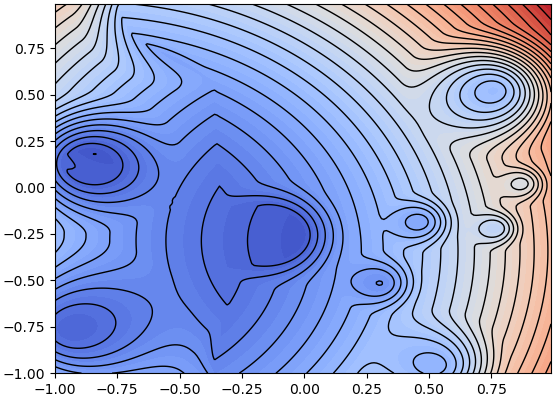
\includegraphics[width=0.7\textwidth]{fig1.png} 
\caption{Contour plots of 2-dimensional convolution.}\label{fig1} 
\end{figure}

The Pareto front in one of test problems is shown in Fig.~\ref{fig2a} and Fig.~\ref{fig2b}. Here Fig.~\ref{fig2a} corresponds to the Pareto front computed on the uniform grid with the step 0.05 in the search domain whereas Fig.~\ref{fig2b} shows the Pareto front computed by RALR-DA.

\begin{figure}
\centering
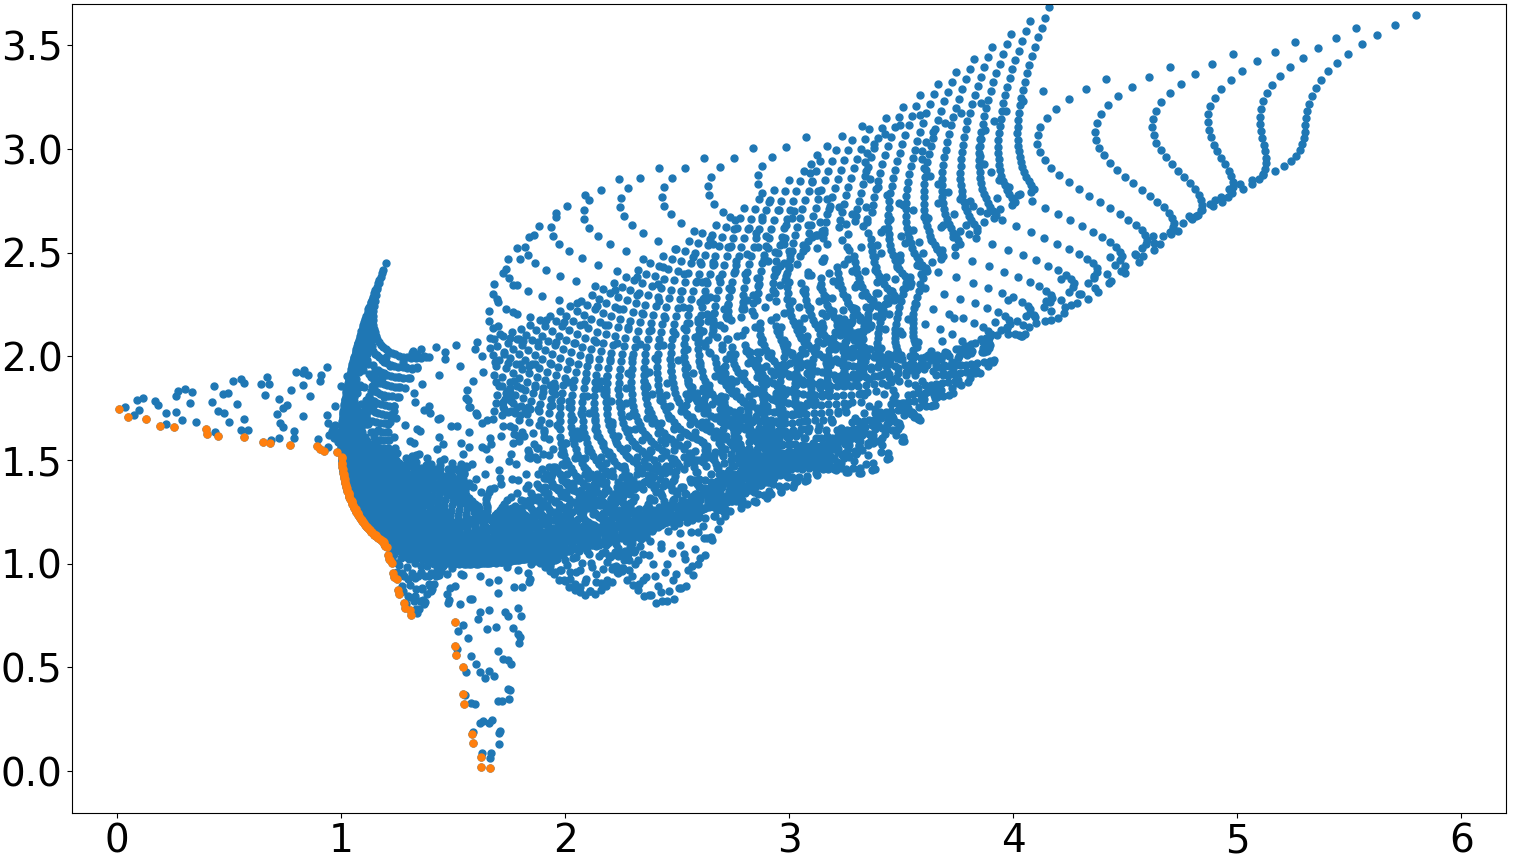
\includegraphics[width=0.7\textwidth]{fig2a.png} 
\caption{Pareto front computed by grid technique.}\label{fig2a} 
\end{figure}

\begin{figure}
\centering
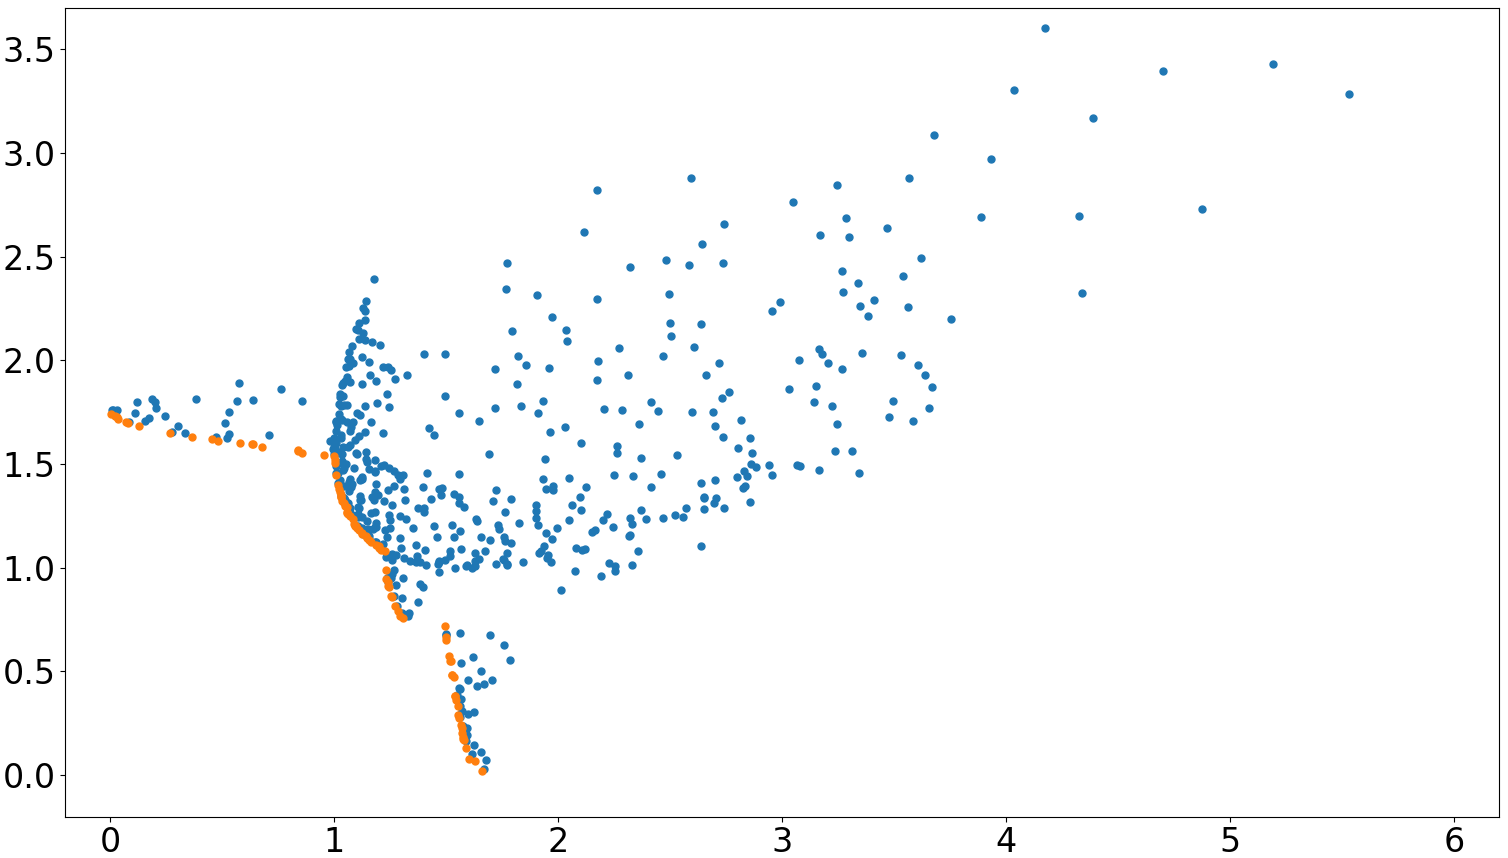
\includegraphics[width=0.7\textwidth]{fig2b.png} 
\caption{Pareto front computed by RALR-DA.}\label{fig2b} 
\end{figure}


The averaged HV indices obtained while solving the two-dimensional bi-criteria problems are presented in Tab.~\ref{tab1} and Fig.~\ref{fig3} where ``Pareto'' corresponds to the estimation obtained by the grid method.

\begin{table}
\caption{Results of the experiment with bi-criteria MCO problems of dimension 2.}
\centering
\begin{tabular}{ccccccc} \hline
 Pareto & RALR-DA & OMOPSO & SMPSO & NSGAII & IBEA & SPEA2 \\ \hline
  6.62 & 6.44 & 5.93 & 5.88 & 5.71 & 5.65 & 5.61 \\ \hline
\end{tabular}
\label{tab1}
\end{table}

\begin{figure}
\centering
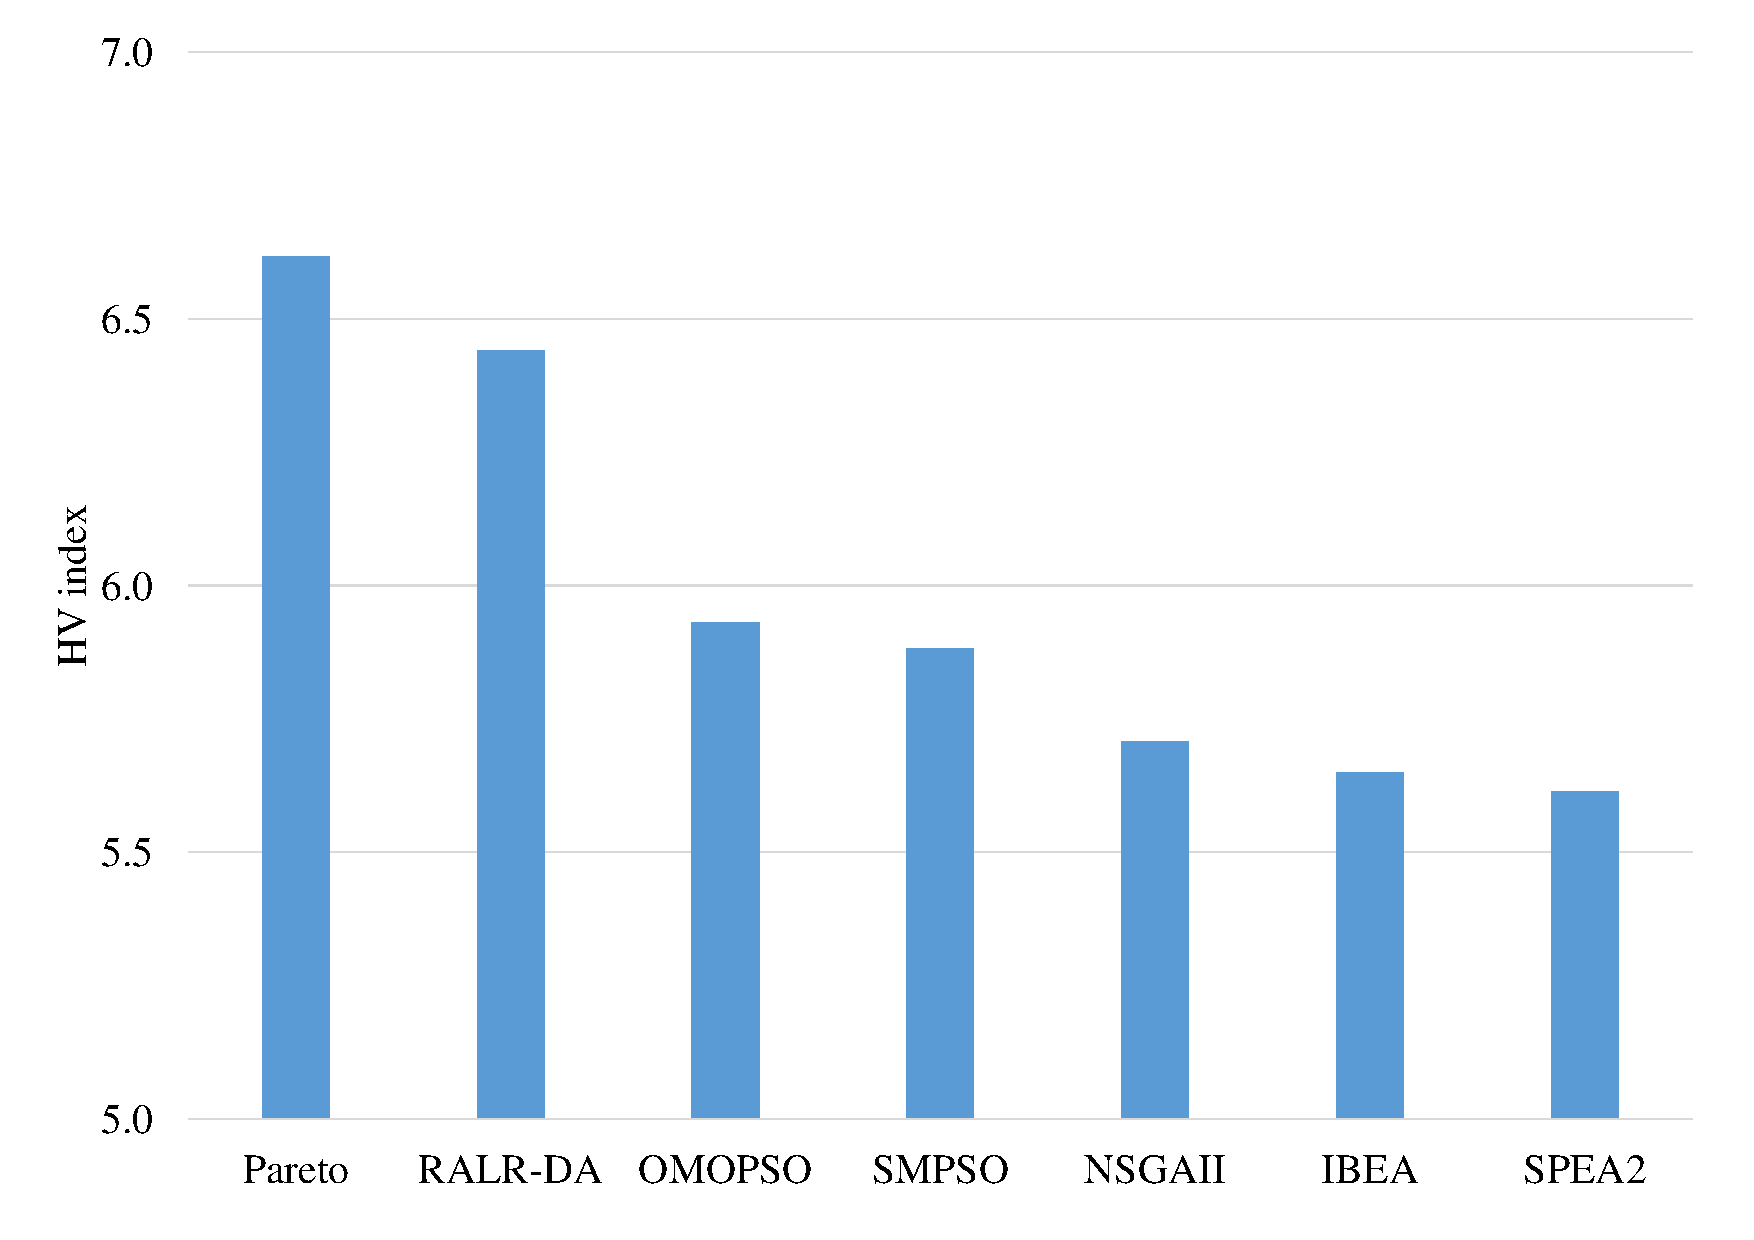
\includegraphics[width=0.7\textwidth]{fig3.pdf} 
\caption{HV indices in bi-criteria 2-dimensional case.}\label{fig3} 
\end{figure}

The second experiment was aimed at solving bi-criteria 4-dimensional MCO problems. 10 test problems have been investigated and for each of them, 100 convolutions (\ref{conv_problem}) with uniformly distributed weight coefficients $\lambda$ were minimized by RALR-DA. 
Tab.~\ref{tab2} contains the results achieved by the methods participated in the experiment and Fig.~\ref{fig4} presents them in graphical form.

\begin{table}
\caption{Results of testing bi-criteria 4-dimensional MCO problems.}
\centering
\begin{tabular}{ccccccc} \hline
 Pareto & RALR-DA & SPEA2 & OMOPSO & IBEA & NSGAII & SMPSO   \\ \hline
  5.04 & 4.71 & 4.53 & 4.45 & 4.39 & 4.39 & 4.37 \\ \hline
\end{tabular}
\label{tab2}
\end{table}

\begin{figure}
\centering
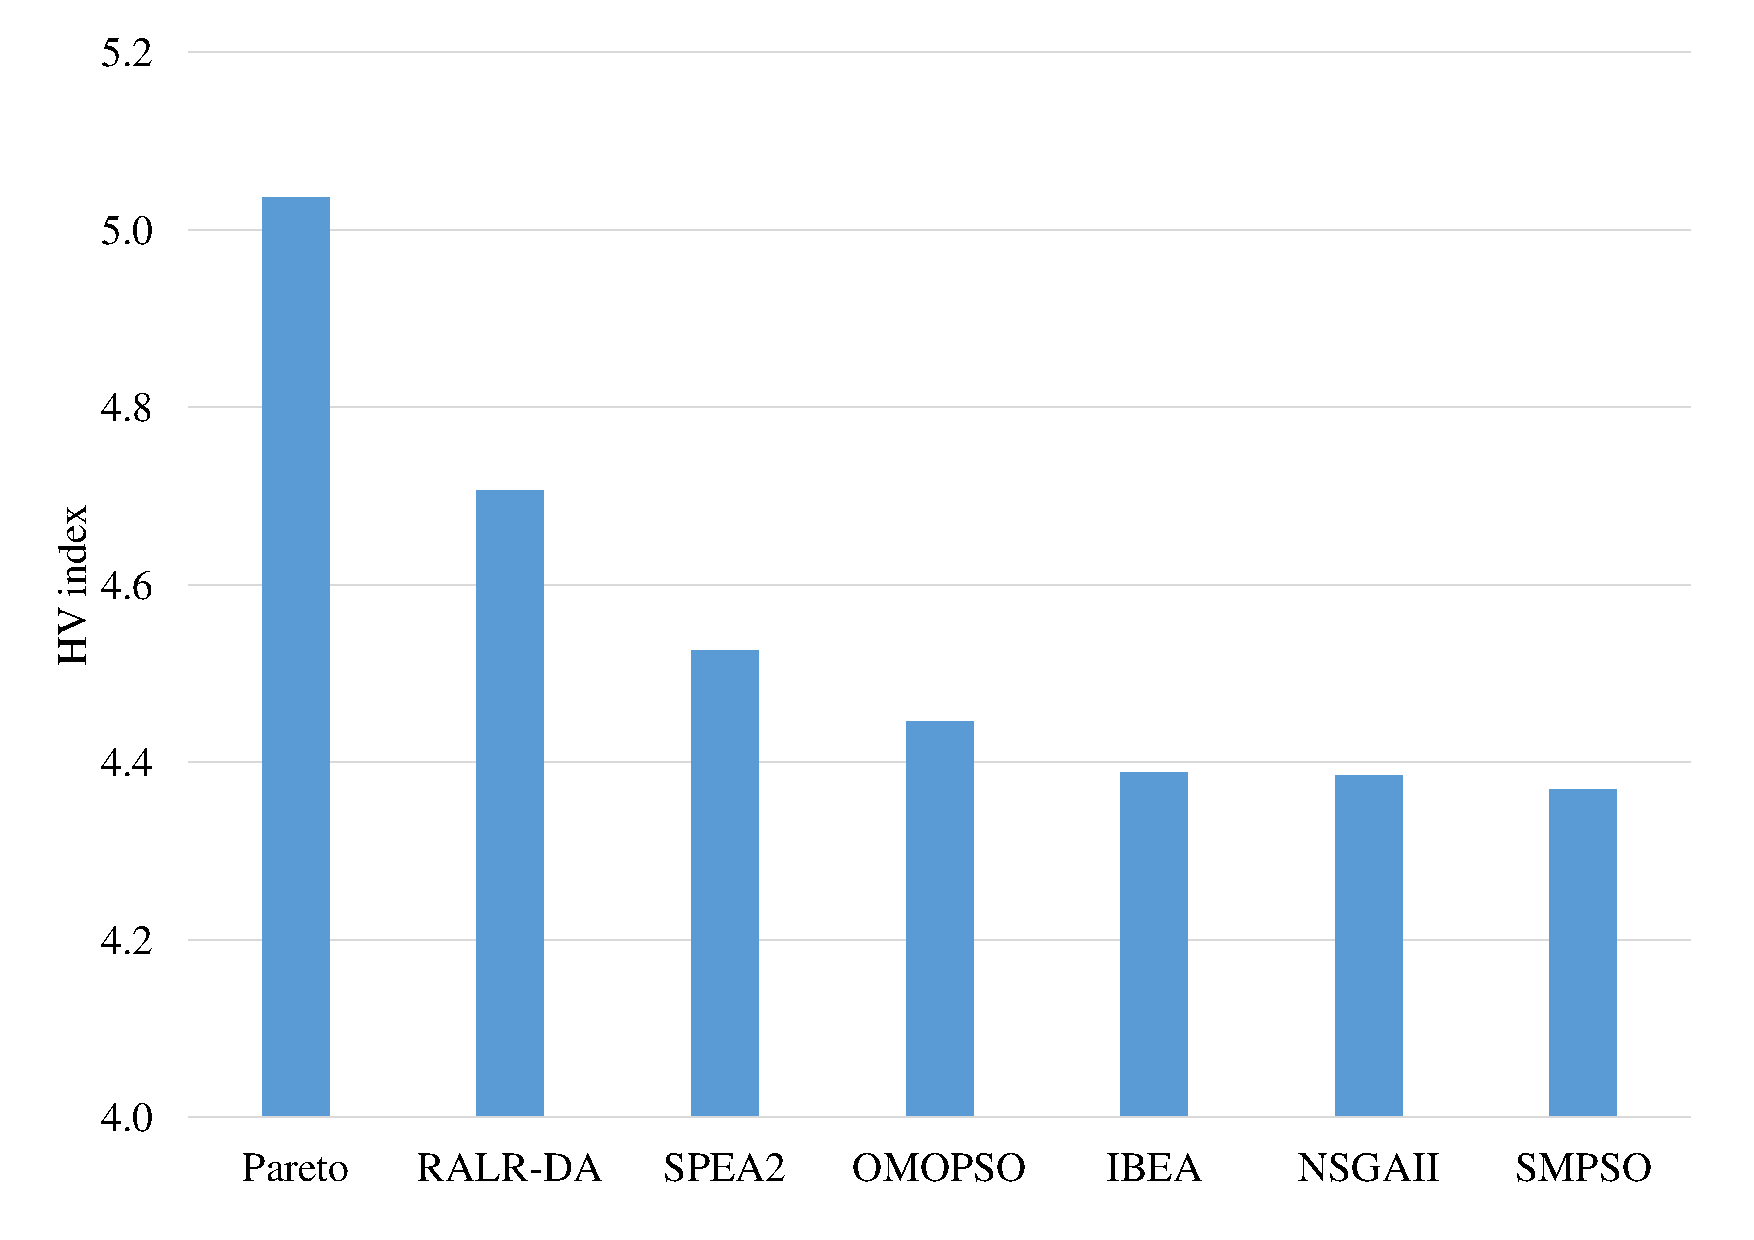
\includegraphics[width=0.7\textwidth]{fig4.pdf} 
\caption{HV indices in bi-criteria 4-dimensional case.}\label{fig4} 
\end{figure}


The third collection of test problems consisted of 10 two-dimensional MCO benchmarks with 4 criteria. In this experiment RALR-DA in each MCO problem minimized convolutions (\ref{conv_problem}) corresponding to 100 different values of weight coefficients $\lambda$ uniformly distributed in the domain (\ref{lambda}).
Like  the  previous experiments, the results are presented in Tab.~\ref{tab3} and Fig.~\ref{fig5}.

\begin{table}
\caption{Results of testing 2-dimensional MCO problems with 4 criteria.}
\centering
\begin{tabular}{ccccccc} \hline
 Pareto & RALR-DA & OMOPSO & SPEA2 & SMPSO & IBEA & NSGAII   \\ \hline
  23.89 & 23.52 & 22.87 & 22.80 & 22.53 & 20.68 & 19.82 \\ \hline
\end{tabular}
\label{tab3}
\end{table}

\begin{figure}
\centering
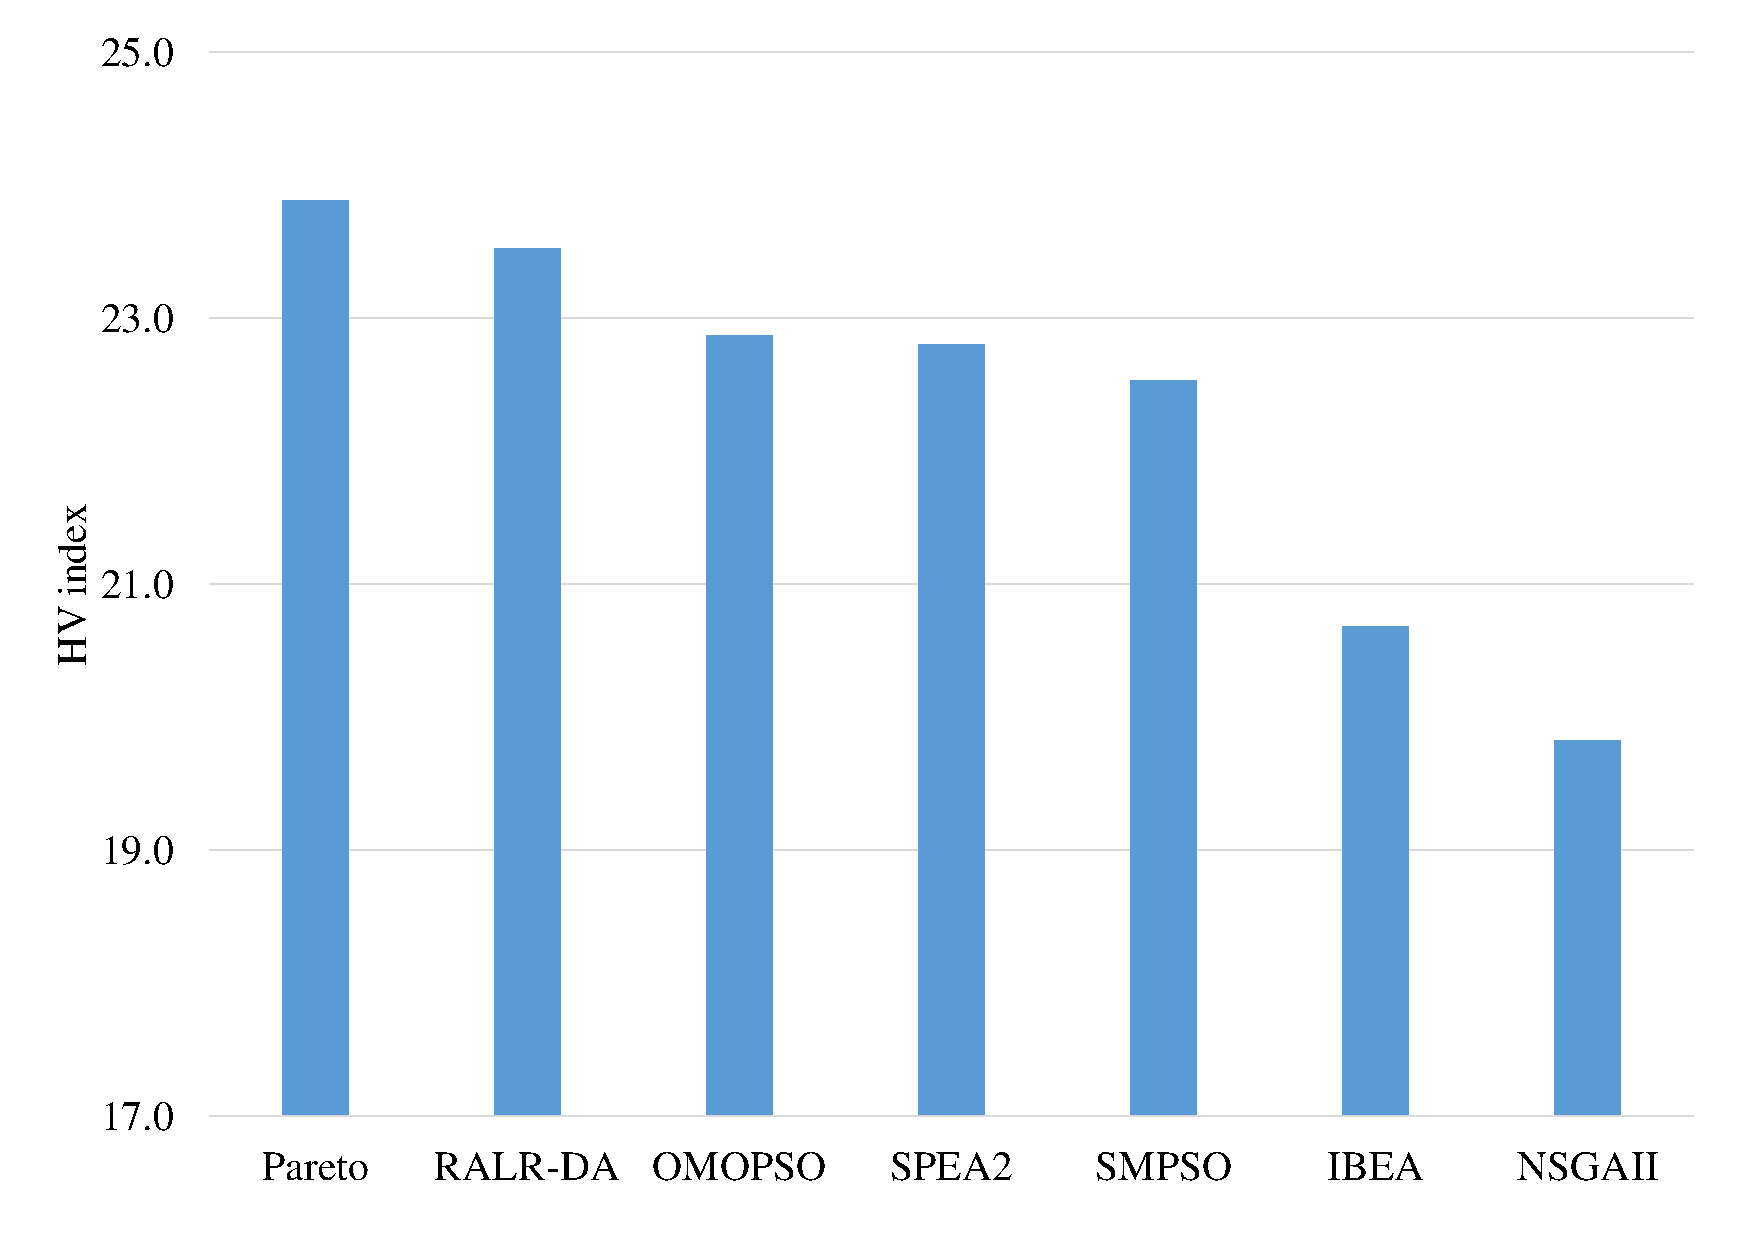
\includegraphics[width=0.7\textwidth]{fig5.pdf} 
\caption{HV indices in 4-criteria 2-dimensional case.}\label{fig5} 
\end{figure}

As it can be seen from the presented experiments, the proposed method demonstrates the best results among all methods involved in evaluation of their effectiveness based on HV index. Moreover, the efficiency of RALR-DA is close to the best one estimated on a dense uniform grid.

As for metaheuristic algorithms, their results differ in different experiments.  For example, in 4-dimensional bi-criteria case the method SPEA is the best among nature-inspired algorithms, but it is the worst in 2-dimensional problems with 2 criteria. On the whole, as the most stable metaheuristic method, the algorithm OMOPSO can be recognized.

\section{Conclusion}

In the paper the multidimensional problems of multicriteria (multiobjective) optimization with black-box time-consuming criteria satisfying the Lipschitz condition are considered. These assumptions lead to significant complexity of the problems under investigation and require the development of special efficient numerical methods for their solving. For this goal in the paper a new algorithm is proposed and its computational scheme is described. The algorithm is based on reducing the MCO problem to a family of single-criterion (scalar) optimization problems generating Pareto-optimal solutions via building parameterized convolutions. In turn, each multidimensional scalar problem is reduced to a univariate one by means of Peano curves that map the multidimensional feasible domain into the real axis. Under Lipschitz condition for criteria the objective functions of the reduced one-dimensional problems satisfy the H{\"o}lder condition and for solving these problems it is necessary to apply specialized global optimization methods. As such method we propose a new algorithm that combines in its decision rule iteration with ``local'' and ``global'' goals. Global iterations provide the convergence to the global optimum and the local ones accelerate the search. Moreover, while solving the univariate problems generated by the family of convolutions the proposed algorithm is able to take into account the criteria values computed already in the course of solving the univariate problems completed earlier. This feature reduces significantly number of trials (calculations of criteria values): the later a problem is solved, the less new criteria computations are produced.

The quality of the proposed algorithm is studied in experiment on 3 representative sets of multiextremal MCO problems of different dimensions and criteria number in comparison with 5 particle swarm and genetic methods. As a criterion of methods' efficiency the hypervolume index estimating the quality of Pareto set approximation is taken. Among all competitors the proposed algorithm demonstrates the best results.

As the directions of further development of the current research it would be interesting to investigate the possibilities of applying other schemes of dimensionality reduction, for example,
the nested optimization scheme \cite{Grishagin2016,Grishagin2018}, the diagonal \cite{Sergeyev2015,Sergeyev2017} or simplicial \cite{Zilinskas2011,PaulaviciusZilinskas2014} partition methods
in the framework of the general approach used in the paper. Moreover, the prospective way is to develop parallel versions of the proposed general scheme oriented at powerful supercomputer systems.


\bibliographystyle{splncs04}
\bibliography{bibliography}

\end{document}
